\section{Einleitung}

In diesem Abschnitt werden einige wichtige Begriffe, die im Laufe des
Dokuments auftauchen werden, kurz erl"autert.

\subsection{Grundlagen von Mesh-Netzen}

\subsubsection{Hintergrund}

Ein drahtloses vermaschtes Netz (engl. Wireless Mesh Network, WMN) besteht
aus einer Menge von Knoten, die "uber drahtlose Kommunikationstechniken
wie beispielsweise IEEE 802.11 (\ref{ieee80211abg}) Nachrichten austauschen. Die
Vemaschung der Knoten erm"oglicht dabei nicht nur den Austausch von
Nachrichten zwischen unmittelbar benachbarten Knoten, sondern auch die
Vermittlung von Nachrichten an entfernte Knoten "uber mehrere Knoten
hinweg. Die Vermittlungsfunktionalit"at wird dabei oft von dedizierten
Vermittlungsknoten (engl. Mesh Router) bereitgestellt, die somit eine
drahtlose Kommunikationsinfrastruktur f"ur die Klienten (engl. Mesh
Client) bilden. Durch den Einsatz vergleichsweise kosteng"unstiger
Hardwarekomponenten und die Vermaschung der Knoten erm"oglichen WMNs die
kosteng"unstige Vernetzung auch gr"o"serer Gebiete. Entsprechende Netze
werden beispielsweise von Community-Projekten wie das Freifunk-Projekt (\ref{other_mesh_projects})
oder Firmen wie Google ((\ref{other_mesh_projects}) bereits heute in der Praxis f"ur den Aufbau gr"o"serer
Netze eingesetzt, um beispielsweise kosteng"unstige Internetzug"ange f"ur
Stadtteile oder ganze St"adte zu realisieren.

WMNs sind auch f"ur den Sonderforschungsbereich (SFB) Nexus an der
Universit"at Stuttgart \cite{nexus} von gro"sem Interesse. Im
Zentrum der Forschungen des SFB stehen Umgebungsmodelle f"ur mobile
kontextbezogene Systeme. Umgebungsmodelle sind digitale Abbilder der
physischen Welt, die von kontextbezogenen Systemen genutzt werden, um
sich selbst"andig an die physische Umgebung des Benutzers anzupassen. Ein
einfaches Beispiel sind ortsbezogene Anwendungen, die beispielsweise
aufgrund der aktuellen geographischen Position eines Ger"ats automatisch
Informationen "uber nahe Restaurants, Sehensw"urdigkeiten, usw. selektieren
k"onnen. Zur Kommunikation, insbesondere mit mobilen Ger"aten, werden dabei
hybride Systeme betrachtet, in denen sowohl eine infrastrukturbasierte
Kommunikation als auch die direkte Ad-hoc-Kommunikation zwischen
mobilen Endsystemen m"oglich ist. Hierbei spielen WMNs als eine spezielle
Auspr"agung eines hybriden Kommunikationssystems eine wesentliche Rolle.


\subsubsection{Ad-Hoc}

Ein Ad-hoc-Netz (lat. ad hoc, sinngem"a"s f"ur diesen Augenblick gemacht)
ist ein drahtloses Rechnernetz, das zwei oder mehr Endger"ate zu einem
vermaschten Netz verbindet. Netze, die sich selbst"andig aufbauen und
konfigurieren, nennt man auch mobile Ad-hoc-Netze (engl. mobile ad hoc
network, MANet) oder Mesh-Netze (engl. mesh, Masche, Netz).

Ad-hoc-Netze verbinden mobile Ger"ate (Netzknoten) wie
Mobiltelefone, Personal Digital Assistants und Notebooks ohne
feste Infrastruktur wie Wireless Access Points. Daten werden von
Netzknoten zu Netzknoten weitergereicht, bis sie ihren Empf"anger
erreicht haben, wodurch sich die Datenlast vorteilhafter verteilt
als in Netzen mit zentraler Anlaufstelle. Knappe Ressourcen
wie Rechenzeit, Energie und Bandbreite fordern eine effektive
Zusammenarbeit der Netzknoten. Spezielle Routingverfahren sorgen
daf"ur, dass sich das Netz best"andig anpasst, wenn sich Knoten
bewegen, hinzukommen oder ausfallen.

\subsubsection{Mesh-Netz}

In einem vermaschten Netz (Mesh-Netz) ist jeder Netzwerkknoten mit einem
oder mehreren anderen verbunden. Die Informationen werden von Knoten
zu Knoten weitergereicht, bis sie das Ziel erreichen. Vermaschte
Netze sind im Regelfall selbstheilend und dadurch sehr zuverl"assig:
Wenn ein Knoten oder eine Verbindung blockiert ist oder ausf"allt, kann
sich das Netz darum herum neu stricken. Die Daten werden umgeleitet und
das Netzwerk ist nach wie vor betriebsf"ahig. 

Vorteile eines vermaschten Funknetzes:
\begin{itemize}
\item Sicherste Variante eines Netzwerkes
\item Bei Ausfall eines Endger"ates ist durch Umleitung die
Datenkommunikation weiterhin m"oglich
\item Sehr leistungsf"ahig
\item Gute Lastverteilung
\item Niedrige Netzwerkkosten
\item Keine zentrale Verwaltung
\end{itemize}

Nachteile eines vermaschten Funknetzes:
\begin{itemize}
\item Vergleichsweise komplexes Routing n"otig
\item Speichern von Routing-Tabellen in jedem Endger"at
\item Jedes Endger"at arbeitet als Router und ist demnach oft aktiv
\item Die Endger"ate sollten m"oglichst eingeschaltet bleiben
\item H"oherer Stromverbrauch im Endger"at
\end{itemize} 

\subsubsection{IEEE 802.11a/b/g}
\label{ieee80211abg}

\textbf{IEEE 802.11} (auch: Wireless LAN, WLAN, WiFi) bezeichnet eine IEEE-Norm
f"ur drahtlose Netzwerkkommunikation. Herausgeber ist das Institute of
Electrical and Electronics Engineers (IEEE).

\textbf{802.11a} spezifiziert eine weitere Variante der physikalischen Schicht,
die im 5-GHz-Band arbeitet und "Ubertragungsraten bis zu 54 MBit/s
ermoglicht. 

\textbf{Vorteile }
\begin{itemize}
	\item weniger genutztes Frequenzband, dadurch h"aufig
	st"orungsfreierer Betrieb m"oglich 
	\item in Deutschland 19 (bei BNetzA-Zulassung) nicht "uberlappende
	Kan"ale 
	\item h"ohere Reichweite, da mit 802.11h bis zu 1000 mW Sendeleistung
	m"oglich 
\end{itemize}

\textbf{Nachteile }
\begin{itemize}
	\item st"arkere Regulierungen in Europa: auf den meisten Kan"alen DFS
	n"otig 
	\item auf einigen Kan"alen kein Betrieb im Freien erlaubt 
	\item falls kein TPC benutzt wird, muss die Sendeleistung reduziert
	werden 
	\item Ad-hoc-Modus wird von den meisten Ger"aten
		nicht unterst"utzt
	\item geringere Verbreitung, daher wenig verf"ugbare Ger"ate
		auf dem Markt und hohe Kosten
\end{itemize}

\textbf{802.11b} ist ebenfalls eine alternative Spezifikation der physikalischen
Schicht, die mit dem bisher genutzten 2,4-GHz-Band auskommt und
"Ubertragungsraten bis zu 11 MBit/s erm"oglicht. 

\textbf{Vorteile}
\begin{itemize}	
	\item gebuhrenfreies freigegebenes ISM-Frequenzband 
	\item hohe Verbreitung und daher geringe Ger"atekosten 
\end{itemize}

\textbf{Nachteile}
\begin{itemize}	
	\item Frequenz muss mit anderen Ger"aten/Funktechniken geteilt werden
	(Bluetooth, Mikrowellenherde, etc.) 
	\item st"orungsfreier Betrieb von nur maximal 3 Netzwerken
	am selben Ort m"oglich, da effektiv nur 3 brauchbare
	(kaum "uberlappende) Kan"ale zur Verf"ugung stehen
	(in Deutschland: 1, 7, 13) 
\end{itemize}

\subsubsection{Ad-Hoc Routing-Protokolle}

Ein Ad-hoc Netzwerk beispielsweise ein Sensornetzwerk besteht aus einer
gro"ser Anzahl von Knoten, die sich typischerweise spontan vernetzen
m"ussen. "Uber Funk k"onnen diese Knoten miteinander kommunizieren. Aber
Knoten kann wegen der Leistungsf"ahigkeit, des Energieverbrauches
und auch der Mobilit"at nicht mit allen anderen Knoten direkt Daten
"ubertragen. Routing Methoden bieten die M"oglichkeit, Kommunikation
zwischen zwei Knoten mit Hilfe der anderen Knoten auszuf"uhren, wenn die
zwei Knoten miteinander nicht direkt kommunizieren k"onnen.

Es gibt mehr als 70 konkurrierende Entw"urfe f�r das Routing der Pakete
durch ein Mobiles Ad-Hoc/Maschennetzwerk. Eine Klassifikation der
Routingprotokolle kann durch Anzahl der Empf"anger getroffen werden:
\begin{itemize}
\item unicast Routing - Ziel der Daten"ubertragung ist ein einzelner Knoten
\item multicast Routing - Ziel sind mehrere Knoten
\item geocast Routing - Ziel sind alle Knoten in einem bestimmten
geografischen Bereich
\item broadcast Forwarding - Ziel sind alle Knoten in der Reichweite
des Senders
\end{itemize}

Eine andere M"oglichkeit der Klassifikation besteht in der Einteilung
der Protokolle hinsichtlich des grunds"atzlichen Ansatzes. Diese Ans"atze
werden im Folgenden vorgestellt.

\textbf{Positionsbasierte Routingverfahren}

Positionsbasierte Routingverfahren nutzen geod"atische Informationen "uber
die genauen Positionen der Knoten. Diese Informationen werden z. B. "uber
GPS-Empf"anger gewonnen. Anhand dieser Ortsinformationen l"asst sich der
k"urzeste oder der beste Pfad zwischen Quell- und Zielknoten bestimmen. Ein
Beispiel f"ur ein positionsbasiertes Routingprotokoll ist LAR.

\textbf{Topologiebasierte Routingverfahren}

Die topologiebasierten Routingverfahren kommen ohne geod"atische
Informationen "uber die Positionen der Knoten des mobilen
Ad-hoc-Netzes aus. Ihnen gen"ugen logische Informationen "uber die
Nachbarschaftsbeziehungen der Knoten, also welche Knoten eine direkte
Verbindung haben oder "uber einen oder mehrere Zwischenknoten (hop)
in Verbindung treten k"onnen. Diese Nachbarknoten k"onnen miteinander
kommunizieren. Die topologischen Informationen werden meistens durch
den Versand so genannter HELLO-Pakete gewonnen. Je nach Zeitpunkt des
Aufbaus der Topologiedatenbasis handelt es sich um proaktives oder
reaktives Routing. Ein Beispiel f"ur ein Protokoll aus dieser Klasse ist
das Neighbourhood Discovery Protocol (NHDP), das Elemente des Optimized
Link State Routing Protocol (OLSR) verwendet.

\textbf{Proaktive Verfahren}

Proaktive Routingverfahren bestimmen die zu verwendenden Pfade zwischen
zwei Knoten bereits, bevor diese f"ur die "Ubertragung von Nutzdaten
ben"otigt werden. Sollen dann Nutzdaten verschickt werden, so muss nicht
auf die Bestimmung des Pfads zum Zielknoten gewartet werden. Nachteilig
ist daf"ur jedoch, dass diese Verfahren auch ohne Verkehr von Nutzdaten
viele Kontrollpakete verschicken, um Pfade zu bestimmen, die wom"oglich
sp"ater nicht ben"otigt werden. Ein Beispiel f"ur ein Protokoll aus dieser
Klasse ist das Optimized Link State Routing Protocol (OLSR).

\textbf{Reaktive Verfahren}

Im Gegensatz zu den proaktiven Verfahren bestimmen reaktive
Routingverfahren f"ur mobile Ad-hoc-Netze die ben"otigten Pfade zwischen
zwei Knoten erst, wenn Nutzdaten "ubertragen werden sollen. Daraus ergibt
sich, dass das erste Datenpaket einer Verbindung erst mit Verz"ogerung
versendet werden kann, da zun"achst auf den Abschluss der Routenbestimmung
gewartet werden muss. Daf"ur werden allerdings auch nur Kontrollpakete
versendet, wenn Nutzdaten verschickt werden und dies zur Routenbestimmung
notwendig ist. Dies schl"agt sich positiv im Energieverbrauch der Knoten
nieder. Das Protokoll Ad hoc On-Demand Distance Vector (AODV) ist ein
Beispiel f"ur ein Protokoll dieser Kategorie.

\textbf{Hybride Verfahren}

Hybride Verfahren kombinieren proaktive und reaktive
Routingverfahren. Dabei soll das Ziel erreicht werden, die
Vorteile der beiden Ans"atze in einem neuen Routingprotokoll
zusammenzufassen. Beispielsweise kann in einem lokal beschr"ankten Bereich
ein proaktives Verfahren eingesetzt werden, w"ahrend f"ur weiter entfernte
Ziele ein reaktives Verfahren eingesetzt wird. Dies vermindert die
Belastung des Netzes durch Kontrollpakete, die bei einem rein proaktiven
Verfahren "uber das gesamte Netz versendet w"urden. Trotzdem stehen f"ur
lokale Ziele sofort Pfade zur Verf"ugung, ohne dass auf deren Bestimmung
wie bei einem rein reaktiven Verfahren gewartet werden m"usste. ZRP ist
ein Routingprotokoll, das diesen Ansatz umsetzt.

\paragraph{OLSR}
\mbox{}
\begin{figure}[H]

\includegraphics{Olsrd_logo.png}
\end{figure}

Optimized Link State Routing, kurz OLSR, ist ein Routingprotokoll
f"ur mobile Ad-hoc-Netze, das eine an die Anforderungen eines mobilen
drahtlosen LANs angepasste Version des Link State Routing darstellt. Es
wurde von der IETF mit dem RFC 3626 standardisiert. Bei diesem
verteilten flexiblen Routingverfahren ist allen Routern die vollst"andige
Netztopologie bekannt, sodass sie von Fall zu Fall den k"urzesten Weg zum
Ziel festlegen k"onnen. Als proaktives Routingprotokoll h"alt es die daf"ur
ben"otigten Informationen jederzeit bereit. Ein in Mesh-Netzwerken
bekannter Vertreter von LSR ist OLSR von olsr.org. Inzwischen existieren
f"ur OLSR spezielle Erweiterungen. Mit der ETX-Erweiterung wird dem
Umstand Rechnung getragen, dass Links asymmetrisch sein k"onnen. Mit
dem Fisheye-Algorithmus ist OLSR auch fur gro"sere Netzwerke brauchbar
geworden, da Routen zu weiter entfernten Knoten weniger h"aufig neu
berechnet werden. Der entscheidende Nachteil ist aber der trotz
Fisheye-Algorithmus noch recht hohe Rechenaufwand von OLSRD, sobald
die Anzahl an Knoten ein gewisses Ma"s ubersteigt.

\paragraph{B.A.T.M.A.N.}
\mbox{}
\begin{figure}[H]
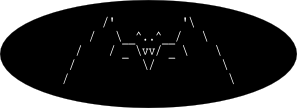
\includegraphics{Batman_logo.png}
\end{figure}

Ausgehend von den Erfahrungen mit Freifunk-OLSR \cite{elektra2007}
begannen die Entwickler
aus der Freifunk-Community im M"arz 2006 in Berlin damit, ein neues
Routingprotokoll f"ur drahtlose Meshnetzwerke zu entwickeln. Alle bisher
bekannten Routingalgorithmen versuchen Routen entweder zu berechnen
(proaktive Verfahren) oder sie dann zu suchen, wenn sie gebraucht werden
(reaktive Verfahren). Das neue Protokoll B.A.T.M.A.N. 
(BETTER APPROACH TO MOBILE ADHOC NETWORKING) \cite{batman} berechnet oder
sucht im Gegensatz zu diesen Protokollen keine Routen, es erfasst
lediglich, ob Routen zu anderen Knoten existieren und "uberwacht ihre
Qualit"at. Dabei interessiert es sich nicht daf"ur, wie eine Route verl"auft,
sondern ermittelt lediglich, "uber welchen direkten Nachbarn ein bestimmter
Netzwerkknoten am besten zu erreichen ist, und tr"agt diese Information
proaktiv in die Routingtabelle ein. 


\subsection{Existierende L"osungen und Projekte}
\label{other_mesh_projects}

\begin{description}

\item[FreiFunk]
hat zum Ziel, freie, unabh"angige und nichtkommerzielle Computer-Funknetze
zu etablieren.  Es bildet eine Plattform f"ur Menschen, die an einer
offenen Netzwerk-Infrastruktur interessiert sind.

\url{http://wiki.freifunk.net/Hauptseite}

\item[OpenNet]
hat sich zur Aufgabe gemacht, freie und offene
Kommunikationsinfrastrukturen zu f"ordern. Dabei setzen die
Vereinsmitglieder auf WLAN-Technik und die Vernetzung von Dach zu Dach
und Haus zu Haus.

\url{http://wiki.opennet-initiative.de/index.php/Hauptseite}

\item[UMIC-Mesh]

ist ein hybrides Testbed f"ur WMNs.
Das Projekt verfolgt 2 Ziele, einerseits ein gro"ses und sklalierbares
Ad-Hoc Mesh-Netzwerk f"ur Forschung bereitzustellen und andererseits
allen Studenten und Mitarbeiter der Computer Science Abteilung
einen breitbandigen Zugang zum Netzwerk der Abteilung zur Verf"ugung zu stellen.

\url{http://umic-mesh.net/}

\item[Google WiFi]

ist ein freies WMN, das von Google finanziert wird und zur Zeit in
Mountain View in Kalifornien eingesetzt wird.

\url{http://wifi.google.com/}

\end{description}
